
\documentclass{exam}

\usepackage{unitsdef} 
\usepackage{graphicx}
% \usepackage[fleqn]{amsmath}
\usepackage{cancel}
\usepackage{float}
\usepackage{mdwlist}
\usepackage{booktabs}
\usepackage{cancel}
\usepackage{polynom}
\usepackage{caption}
\usepackage{fullpage}
\usepackage{enumerate}

% \newcommand{\degree}{\ensuremath{^\circ}} 
\everymath{\displaystyle}

\newunit{\inch}{in}
\newunit{\foot}{ft}
\newunit{\cemtimeter}{cm}

% \begin{figure}[H]
%   \centering
%   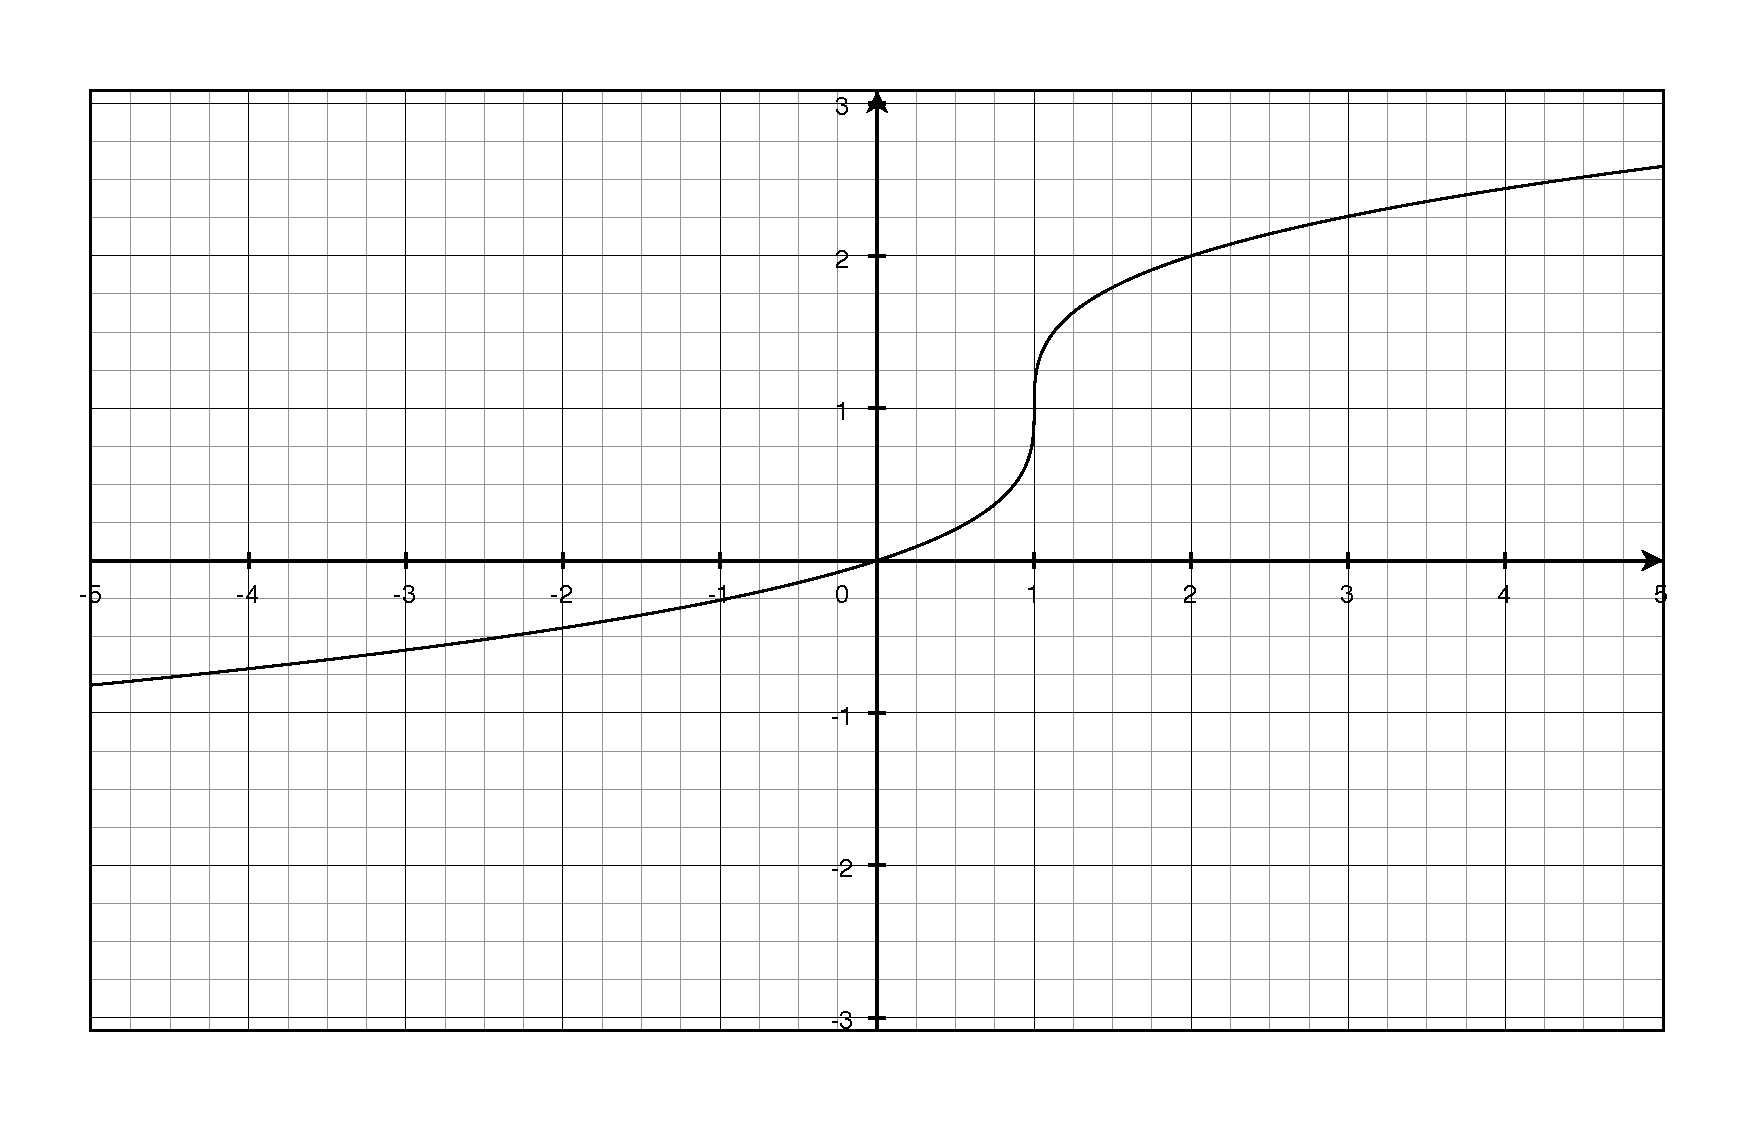
\includegraphics[scale=.3]{question7.eps}
%   \caption*{Question 7}
% \end{figure}

% \begin{tabular}{cc}
% \toprule
% period & amplitude \\
% \midrule
%   $\pi$ & $2$ \\
% \bottomrule
% \end{tabular}

\printanswers

\ifprintanswers 
\usepackage{2in1, lscape} 
\fi

\title{Math 263B \\ Homework Two}
\date{July 19, 2012}

\begin{document}

\maketitle

\section{Homework}

\begin{itemize*}
  \item Read Section 5.2
  \item pp 245-246: 1-14, 17-18, 21-22, 26, 28-29
\end{itemize*}

\section{Extra Credit}
page 245, problem 37

\begin{solution}
For the second part of the flight, we can use the reasoning from problem
22 to find the velocity with which the ball bounces off the floor:
\begin{align*}
  h_{max} &= \frac{v_0^2}{2g} \\
  v_0 &= \sqrt{2gh} \\
      &= \sqrt{2 \cdot 32 \cdot 9} \\
      &= \sqrt{2 \cdot 32 \cdot 9} \\
      &= 24 \foot / \second \\
\end{align*}
\begin{enumerate}[a]

\item
The formulas for the second part of the flight, with $t = 0$ when the ball hits the floor, are:
\begin{align*}
  v &= -32t + 24 \\
  h &= -16t^2 + 24t \\
\end{align*}

The formulas for the first part of the flight, with $t = 0$ when the ball is dropped are:
\begin{align*}
  v &= -32t \\
  h &= -16t^2 + 16 \\
\end{align*}
Actuall, $t = 0$ when the ball is dropped, so we need to figure out how long it takes for the ball to hit the floor:
\begin{align*}
  0 &= -16t^2 + 16 \\
  t &= 1 \second \\
\end{align*}

\pagebreak

So the formulas for the second part of the flight, with the correct time, are:
\begin{align*}
  v &= -32(t - 1) + 24 \\
    &= -32t + 56 \\
  h &= -16(t - 1)^2 + 24(t - 1) \\
    &= -16(t^2 - 2t + 1) + 24t - 24 \\
    &= -16t^2 + 56t - 40 \\
\end{align*}

\item
The first time the ball is at 9 feet is shortly after it is dropped.  We use the formula for the first part of the
flight for this:
\begin{align*}
  9 &= -16t^2 + 16 \\
  t &= \frac{\sqrt{7}}{4} \\
    &\approx 0.66 \second \\
\end{align*}
The next time the ball is at 9 feet is at the peak of the second part of the flight.  The easiest way to find the time
is to find the point when the velocity is zero:
\begin{align*}
    -32t + 56 &= 0 \\
    t &= 1.75 \second \\
\end{align*}

\end{enumerate}

\end{solution}

\ifprintanswers
\pagebreak

\section{Section 5.2}

\begin{description}
\item[1]
\begin{align*}
  y &= \left( 1 - x^2 \right)^{1/2} \\
  \frac{dy}{dx} &= \frac{1}{2} \left( 1 - x^2 \right)^{-1/2} \cdot (-2x) \\
  &= \frac{-x}{\sqrt{1 - x^2}} \\
\\
  \frac{dy}{dx} + \frac{x}{y} &= \frac{-x}{\sqrt{1 - x^2}} + \frac{x}{\sqrt{1 - x^2}} = 0 \\
\end{align*}

\item[2]
\begin{align*}
  y &= Cx \\
 \frac{dy}{dx} &= C \\
\\
  -x \frac{dy}{dx} + y &= -Cx + Cx = 0 \\
\end{align*}

\item[3]
\begin{align*}
  y &= C_1 \sin x + C_2 \cos x \\
  \frac{dy}{dx} &= C_1 \cos x - C_2 \sin x \\
  \frac{d^2y}{dx^2} &= -C_1 \sin x - C_2 \cos x \\
\\
  \frac{d^2y}{dx^2} + y &= -C_1 \sin x - C_2 \cos x + C_1 \sin x + C_2 \cos x = 0 \\
\end{align*}

\item[4]
\begin{align*}
  y &= \sin(x + C) \\
  \frac{dy}{dx} &= \cos(x + C) \\
\\
  \left( \frac{dy}{dx} \right)^2 + y^2 &= \cos^2(x + C) + \sin^2(x + C) = 1 \\
\end{align*}

\begin{align*}
  y &= \pm 1 \\
  \frac{dy}{dx} &= 0 \\
\\
  \left( \frac{dy}{dx} \right)^2 + y^2 &= 0^2 + (\pm 1)^1 = 1 \\
\end{align*}

\item[5]
\begin{align*}
  \frac{dy}{dx} &= x^2 + 1 \\
  \int \, \mathrm{d}y &= \int \left( x^2 + 1 \right) \, \mathrm{d}x \\
  y &= \frac{1}{3} x^3 + x + C \\
\\
  1 &= \frac{1}{3} 1^3 + 1 + C \\
  C &= - \frac{1}{3} \\
\\
  y &= \frac{1}{3} x^3 + x - \frac{1}{3} \\
\end{align*}

\item[6]
\begin{align*}
  \frac{dy}{dx} &= x^{-3} + 2 \\
  \int  \, \mathrm{d}y &= \int \left( x^{-3} + 2 \right) \, \mathrm{d}x \\
  y &= -\frac{1}{2}x^{-2} + 2x + C \\
\\
  3 &= -\frac{1}{2} + 2 + C \\
  C &= \frac{3}{2} \\
\\
  y &= -\frac{1}{2}x^{-2} + 2x + \frac{3}{2} \\
\end{align*}

\item[7]
\begin{align*}
  \frac{dy}{dx} &= \frac{x}{y} \\
  \int y \, \mathrm{d}y &= \int x \, \mathrm{d}x \\
  \frac{1}{2} y^2 &= \frac{1}{2} x^2 + C \\
  y^2 &= x^2 + C \\
\\
  1 &= 1 + C \\
  C &= 0 \\
\\
  y^2 &= x^2 \\
\end{align*}

\item[8]
\begin{align*}
  \frac{dy}{dx} &= \left( \frac{x}{y} \right)^{1/2} \\
  \frac{dy}{dx} &= \frac{x^{1/2}}{y^{1/2}} \\
  \int y^{1/2} \, \mathrm{d}y &= \int x^{1/2} \, \mathrm{d}x \\
  \frac{2}{3} y^{3/2} &= \frac{2}{3} x^{3/2} + C \\
  y^{3/2} &= x^{3/2} + C \\
\\
  4^{3/2} &= 1 + C \\
  C &= 7 \\
\\
  y^{3/2} &= x^{3/2} + 7 \\
\end{align*}

\item[9]
\begin{align*}
  \frac{dz}{dt} &= t^2z^2 \\  
  \int z^{-2} \, \mathrm{d}z &= \int t^2 \, \mathrm{d}t \\
  -z^{-1} &= \frac{1}{3} t^3 + C \\
  %% z^{-1} &= -\frac{1}{3} t^3 + C \\
  %% \frac{3}{z} &= -t^3 + C \\
  z &= \frac{3}{-t^3 + C} \\
\\
  \frac{1}{3} &= \frac{3}{-1 + C} \\
  -1 + C &= 9 \\
  C &= 10 \\
\\
  z &= \frac{3}{10 - t^3} \\
\end{align*}

 \item[10]
\begin{align*}
  \frac{dy}{dt} &= y^4 \\  
  \int y^{-4}\, \mathrm{d}y &= \int \, \mathrm{d}t \\
  - \frac{1}{3} y^{-3} &= t + C \\
  % \frac{1}{3y^3} &= -t + C \\
  y^3 &= \frac{-1}{3t + C} \\
\\
  1 &= \frac{-1}{C} \\
  C &= -1 \\
\\
  y^3 &= \frac{-1}{3t - 1} \\
\end{align*}

\item[11]
\begin{align*}
  \frac{ds}{dt} &= 16t^2 + 4t - 1 \\  
  \int \, \mathrm{d}s &= \int \left( 16t^2 + 4t - 1 \right) \, \mathrm{d}t \\
  s &= \frac{16}{3} t^3 + 2t^2 - t + C \\
\\
  100 &= C \\
\\
  s &= \frac{16}{3} t^3 + 2t^2 - t + 100 \\
\end{align*}

\item[12]
\begin{align*}
  \frac{du}{dt} &= u^3 \left( t^3 - t \right) \\  
  \int u^{-3} \, \mathrm{d}u &= \int \left( t^3 - t \right) \, \mathrm{d}t \\
  - \frac{1}{2} u^{-2} &= \frac{1}{4} t^4 - \frac{1}{2} t^2 + C \\
  % \frac{2}{u^2} &= -t^4 + 2t^2 + C \\
  u^2 &= \frac{2}{-t^4 + 2t^2 + C} \\
\\
  1 &= \frac{2}{C} \\
  C &= 2 \\
\\
  u^2 &= \frac{2}{-t^4 + 2t^2 + 2}
\end{align*}

\item[13]
\begin{align*}
  \frac{dy}{dx} &= \left( 2x + 1 \right)^4 \\  
  \int \, \mathrm{d}y &= \int \left( 2x + 1 \right)^4 \, \mathrm{d}x \\
  y &= \frac{1}{10} \left( 2x + 1 \right)^5 + C \\
\\
  6 &= \frac{1}{10} + C \\
  C &= \frac{59}{10} \\
\\
  y &= \frac{1}{10} \left( 2x + 1 \right)^5 + \frac{59}{10} \\
\end{align*}

\item[14]
\begin{align*}
  \frac{dy}{dx} &= -y^2 x \left(x^2 + 2 \right)^4 \\  
  - \int y^{-2} \, \mathrm{d}y &= \int \left( x^2 + 2 \right)^4 x \, \mathrm{d}x \\
  y^{-1} &= \frac{1}{10} \left( x^2 + 2 \right)^5 + C \\
  % \frac{1}{y} &= \frac{\left( x^2 + 2 \right)^5}{10} + C \\
  y &= \frac{10}{\left( x^2 + 2 \right)^5 + C} \\
\\
  1 &= \frac{10}{2^5 + C} \\
  % 32 + C &= 10 \\
  C &= -22 \\
\\
  y &= \frac{10}{\left( x^2 + 2 \right)^5 - 22} \\
\end{align*}

\item[17]
Find an equation for the velocity:
\begin{align*}
  \frac{dv}{dt} &= t \\
  \int  \, \mathrm{d}v &= \int t \, \mathrm{d}t \\
  v &= \frac{1}{2} t^2 + C \\
\end{align*}

Use the initial conditions to find the value of the constant:
\begin{align*}
  3 &= 0 + C \\
  C &= 3 \\
\end{align*}

Find an equation for the position:
\begin{align*}
  \frac{ds}{dt} &= \frac{1}{2} t^2 + 3 \\
  \int \, \mathrm{d}s &= \int \frac{1}{2} t^2 + 3 \, \mathrm{d}t \\
  s &= \frac{1}{6} t^3 + 3t + C \\
\end{align*}

Use the initial conditions to find the value of the constant:
\begin{align*}
  0 &= 0 + C \\
  C &= 0 \\
\end{align*}

The final equations are:
\begin{align*}
  v &= \frac{1}{2} t^2 + 3 \\
  s &= \frac{1}{6} t^3 + 3t \\
\end{align*}

Find the values at time 2:
\begin{align*}
  v(2) &= 5 \cm / \second \\
  s(2) &= \frac{22}{3} \cm \\
\end{align*}

\item[18]
Find an equation for the velocity:
\begin{align*}
  \frac{dv}{dt} &= (1 + t)^{-4} \\
  \int  \, \mathrm{d}v &= \int (1 + t)^{-4} \, \mathrm{d}t \\
  v &= -\frac{1}{3} (1 + t)^{-3} + C_1 \\
\end{align*}

Use the initial conditions to find the value for the constant:
\begin{align*}
  0 &= -\frac{1}{3} + C_1 \\
  C_1 &= \frac{1}{3} \\
  v &= -\frac{1}{3} (1 + t)^{-3} + \frac{1}{3} \\
\end{align*}

Find an equation for the position:
\begin{align*}
  \frac{ds}{dt} &= -\frac{1}{3} (1 + t)^{-3} + \frac{1}{3} \\
  \int \, \mathrm{d}s &= \int \left[ -\frac{1}{3} (1 + t)^{-3} + \frac{1}{3} \right] \, \mathrm{d}t \\
  s &= \frac{1}{6} (1 + t)^{-2} + \frac{1}{3} t + C_2 \\
\end{align*}

Use the initial conditions to find the value for the constant:
\begin{align*}
  10 &= \frac{1}{6} + \frac{1}{3} t + C_2 \\
  C_2 &= \frac{19}{2} \\
  s &= \frac{1}{6} (1 + t)^{-2} + \frac{1}{3} t + \frac{19}{2} \\
\end{align*}

Find the velocity and position at time 2:
\begin{align*}
  v(2) &= -\frac{1}{3} (3)^{-3} + \frac{1}{3} \approx 0.321  \cm / \second \\
  s(2) &= \frac{1}{6} (3)^{-2} + \frac{1}{3} \cdot 2 + \frac{19}{2} \approx 10.185  \cm \\
\end{align*}

\pagebreak

\item[21]
The acceleration of gravity is $-32 \foot / \second^2$.

\begin{align*}
  \frac{dv}{dt} &= -32 \\
  v &= -32t + v_0t \\
\end{align*}

For this problem, $v_0 = 96 \foot / \second$.  The ball is at its peak when the velocity is zero.
\begin{align*}
  v &= -32t + 96 \\
  0 &= -32t + 96 \\
  t &= 3 \second \\
\end{align*}

Now we need an equation for the height:
\begin{align*}
  \frac{dh}{dt} &= -32t + 96 \\
  h &= -16t^2 + 96t + h_0 \\
\end{align*}

Since the ball is thrown from ground level, $h_0 = 0$.  The height at time 3 is:
\[
  h = -16 \cdot 9 + 96 \cdot 3 = 144 \foot \\
\]

\item[22]
Find an equation for the velocity:
\begin{align*}
  \frac{dv}{dt} &= k \\
  v &= kt + v_0 \\
\end{align*}

The peak is reached when the velocity is zero:
\begin{align*}
  0 &= kt + v_0 \\
  -kt &= v_0 \\
  t &= - \frac{v_0}{k} \\
\end{align*}

Find an equation for the height:
\begin{align*}
  \frac{dh}{dt} &= kt + v_0 \\
  h &= \frac{1}{2} kt^2 + v_0 t \\
\end{align*}

Plug in the time to see what the height is:
\begin{align*}
  h_{max} &= \frac{1}{2} k \left( - \frac{v_0}{k} \right)^2 + v_0 \cdot \left( - \frac{v_0}{k} \right) \\
         &= \frac{v_0^2}{2k} - \frac{v_0^2}{k} \\
         &= - \frac{v_0^2}{2k} \\
\end{align*}

\item[26]
The velocity equation is: $v = -32t$.  We need to find out how long it takes the ball to get to reach the desired velocity:

\begin{align*}
  -136 &= -32t \\
  t &= 4.25 \second \\
\end{align*}

The height equation is: $h = -16t^2 - 32t + h_0$.  The final height is zero, so we need to solve for the initial height:

\begin{align*}
  0 &= -16 \cdot (4.25)^2 - 32 \cdot (4.25) + h_0 \\
  h_0 &= 425 \foot \\
\end{align*}

\pagebreak

\item[28]
Find an expression for the velocity:
\begin{align*}
  \frac{dv}{dt} &= -11 \\
  v &= -11t + 60 \\
\end{align*}

Find out how long it takes for the velocity to get to zero:
\begin{align*}
  0 &= -11t + 60 \\
  t &\approx 5.45 \second \\
\end{align*}

Find an expression for the position:
\begin{align*}
  \frac{dx}{dt} &= -11t + 60 \\
  x &= -5.5t^2 + 60t \\
\end{align*}

See how far the car travels in 5.45 seconds:
\begin{align*}
  x &= -5.5 \cdot (5.45)^2 + 60 \cdot 5.45 \\
    &\approx 164 \foot \\
\end{align*}

\item[29]
Find an expression for the velocity:
\begin{align*}
  \frac{dv}{dt} &= a \\
  v &= at + v_0 \\
\end{align*}

Plug in velocities and time and solve for the acceleration:
\begin{align*}
  60 &= 10a + 45 \\
  10a &= 15 \\
  a   &= 1.5 \text{ mph / s}\\
\end{align*}



\end{description}

\else

\vspace{9 cm}

{\em It's peculiar and unnerving in a way to see so many young people walking around with cellphones and iPods in their ears
and so wrapped up in media and video games. It robs them of their self-identity. It's a shame to see them so tuned out
to real life. Of course they are free to do that, as if that's got anything to do with freedom. The cost of liberty is
high, and young people should understand that before they start spending their life with all those gadgets.}
\vspace{.2 cm}

\hspace{1 cm} --Bob Dylan

\fi

\end{document}

